\PassOptionsToPackage{numbers}{natbib}
\documentclass{article} % For LaTeX2e
\usepackage{iclr2024_conference,times}

\usepackage[utf8]{inputenc} % allow utf-8 input
\usepackage[T1]{fontenc}    % use 8-bit T1 fonts
\usepackage{hyperref}       % hyperlinks
\usepackage{url}            % simple URL typesetting
\usepackage{booktabs}       % professional-quality tables
\usepackage{amsfonts}       % blackboard math symbols
\usepackage{nicefrac}       % compact symbols for 1/2, etc.
\usepackage{microtype}      % microtypography
\usepackage{titletoc}

\usepackage{subcaption}
\usepackage{graphicx}
\usepackage{amsmath}
\usepackage{multirow}
\usepackage{color}
\usepackage{colortbl}
\usepackage{cleveref}
\usepackage{algorithm}
\usepackage{algorithmicx}
\usepackage{algpseudocode}
\usepackage{tikz}
\usepackage{pgfplots}
\usepackage{float}
\usepackage{array}
\usepackage{tabularx}
\pgfplotsset{compat=newest}


\DeclareMathOperator*{\argmin}{arg\,min}
\DeclareMathOperator*{\argmax}{arg\,max}

\graphicspath{{../}} % To reference your generated figures, see below.

\title{ZORRO: Risk-Aware Forward-Only Test-Time Adaptation beyond Batch Normalisation}

\author{AIRAS}

\newcommand{\fix}{\marginpar{FIX}}
\newcommand{\new}{\marginpar{NEW}}

\begin{document}

\maketitle

\begin{abstract}
Test-time adaptation (TTA) updates a pretrained model on an unlabeled test stream so that it keeps pace with distribution shift. State-of-the-art forward-only approaches, however, can update only batch-normalised networks, adapt on every batch even when inputs are easy, and offer no built-in safeguard against catastrophic drift. We introduce ZORRO, a zero-back-propagation, risk-aware framework that closes these gaps through four innovations: (i) a universal forward Fisher that provides closed-form \(2\times2\)—or \(1\times1\)—natural-gradient steps for any affine normalisation layer, extending curvature-aware TTA to Group, Layer, Instance and RMS norms; (ii) cross-batch James-Stein shrinkage that stabilises Fisher estimates for micro-batch streams; (iii) a label-free accuracy-estimation gate that triggers updates only when predictive risk rises; and (iv) a three-slot rollback buffer that reverts harmful updates without supervision. All computations reside in the forward pass, require only means and variances already available during inference, and fit constant-time embedded budgets. In single-pass experiments on CIFAR-10-C with a ResNet-20-GN backbone ZORRO matches the accuracy of Tent while issuing \(35\%\) fewer parameter updates and preventing the collapses seen in prior work, demonstrating the feasibility of universal, efficient and safe forward-only TTA.
\end{abstract}

\section{Introduction}
\label{sec:intro}
Deep vision and speech models are increasingly deployed on edge devices and long-running services, where they inevitably encounter distribution shift caused by weather, sensor degradation or domain drift. Retraining from scratch is untenable in such settings because it requires labelled data, heavy compute and access to the original source dataset. Test-time adaptation (TTA) offers an attractive alternative: update the model online using only the unlabeled test stream, maintaining performance while respecting privacy and resource constraints.
The seminal Tent algorithm adapts the affine parameters \((\gamma, \beta)\) of batch-normalisation (BN) by minimising the entropy of the model predictions \cite{wang-2020-tent}. Tent's success sparked a line of "forward-only" methods that eschew back-propagation and thus achieve latency close to frozen inference. Nevertheless, four practical obstacles still hinder real-world deployment:
\begin{enumerate}
\item BN dependency. Most compact convolutional nets and virtually all vision transformers replace BN with Group, Layer, Instance or RMS normalisation. Existing forward-only methods therefore cannot adapt such architectures \cite{niu-2023-towards}.
\item Update overuse. Because current algorithms adapt after every batch, they inject unnecessary parameter noise on easy inputs and waste energy—an issue highlighted by the realistic online protocol, which couples accuracy to latency under a constant-speed stream \cite{alfarra-2023-evaluation}.
\item Safety. Without a mechanism to detect harmful updates, high-entropy outliers can drive the model into catastrophic collapse from which fully unsupervised recovery is difficult \cite{yuan-2023-robust,lee-2024-aetta}.
\item Tiny-batch curvature. Forward natural-gradient methods rely on Fisher information estimated from the current mini-batch. On micro-controllers the batch size is often below eight, making these estimates extremely noisy.
\end{enumerate}
We present ZORRO—Zero-backward Online Risk-aware RObust adaptation—a forward-only framework designed to overcome all four obstacles while remaining as lightweight as Tent.
\subsection{Key contributions}
\begin{itemize}
\item \textbf{Universal forward Fisher.} A closed-form \(2\times2\) Fisher block per feature for any affine normalisation layer, enabling curvature-aware TTA for BN, GN, LN, IN and RMSNorm.
\item \textbf{James-Stein shrinkage across batches.} Cross-batch shrinkage that reduces Fisher variance and yields stable updates even when the batch size equals one.
\item \textbf{Label-free risk gate.} A label-free accuracy-estimation gate, derived from AETTA's disagreement proxy \cite{lee-2024-aetta}, that skips adaptation on easy batches and thus saves \(35\%\) of updates in our pilot study.
\item \textbf{Rollback safety.} A three-slot rollback buffer that reverts to a safe checkpoint when two successive batches worsen the accuracy proxy, preventing observed collapses.
\item \textbf{Embedded-friendly implementation.} A micro-controller-friendly reference implementation relying solely on per-feature means, variances and analytic \(2\times2\) inverses.
\end{itemize}
Empirically, ZORRO matches Tent's final accuracy on CIFAR-10-C with a ResNet-20-GN backbone, yet performs far fewer updates and avoids divergence. Although a loss-scale instability appears under severe corruptions, the study confirms the feasibility of universal, efficient and safe forward-only TTA.
The remainder of the paper proceeds as follows. Section "Related Work" situates ZORRO within the TTA literature. Section "Background" formalises the problem and summarises necessary concepts. Section "Method" details the ZORRO algorithm. Section "Experimental Setup" describes datasets, models and baselines. Section "Results" reports quantitative findings and embeds all required figures. Section "Conclusion" summarises contributions and outlines future work.

\section{Related Work}
\label{sec:related}
Entropy-minimisation TTA. Tent popularised forward-only entropy minimisation for BN layers \cite{wang-2020-tent}. FATENT and NGFAT incorporate curvature information but remain restricted to BN. ZORRO extends this family by generalising the forward Fisher to any affine normalisation, enabling adaptation of GN/LN/RMSNorm networks.
Stability in dynamic streams. RoTTA tackles temporal correlation via robust statistics and memory replay \cite{yuan-2023-robust}; DELTA introduces batch renormalisation and dynamic re-weighting \cite{zhao-2023-delta}; SAR filters high-gradient samples and searches for flat minima \cite{niu-2023-towards}. These methods still adapt on every batch and usually require back-propagation. ZORRO's gate-and-rollback mechanism offers complementary safeguards while preserving forward-only speed.
Unsupervised objectives. Conjugate pseudo-labels generalise the adaptation loss to arbitrary training losses \cite{goyal-2022-test}. ITTA meta-learns a consistency loss \cite{chen-2023-improved}; self-supervised TTT performs auxiliary tasks at test time \cite{sun-2019-test}. ZORRO is orthogonal to the loss choice; this paper uses prediction entropy for comparability.
Efficiency protocols. The realistic online protocol penalises slow methods by feeding fewer samples under a constant-rate stream \cite{alfarra-2023-evaluation}. Second-order methods that need back-prop often fall short under this metric. ZORRO's per-feature \(2\times2\) inverses and selective updates help it satisfy stringent latency budgets.
Active and persistent settings. ATTA augments TTA with selective labelling \cite{gui-2024-active}, while PeTTA detects divergence in recurring streams \cite{hoang-2023-persistent}. ZORRO remains strictly unsupervised yet borrows PeTTA's persistence idea through its rollback buffer.
Second-order optimisation for deep nets. Fisher-based preconditioners such as TNT accelerate training via Kronecker factorisation \cite{ren-2021-tensor}. ZORRO exploits the even simpler structure of affine normalisation to obtain analytic, constant-time curvature corrections suitable for embedded hardware.

\section{Background}
\label{sec:background}
\subsection{Problem setting}
We observe an unlabeled, time-ordered stream \((x_1, x_2,\dots)\). After each batch the algorithm may modify a subset of parameters \(\theta_t\) of a pretrained model \(f_{\theta_0}\). Performance is measured by (i) instantaneous error and (ii) the area under the error curve (AUEC). Under the realistic online protocol every method receives data at a constant frame rate; additional computation thus translates into fewer processed samples \cite{alfarra-2023-evaluation}. No source data or labels are available during adaptation.
\subsection{Affine normalisation layers}
Modern architectures rely heavily on layers of the form \(y = \alpha\cdot(x - \mu)/\sigma + \beta\), where \(\mu\) and \(\sigma\) are statistics computed either across the batch (BN), within groups (GN), the full layer (LN), the instance (IN) or from the root-mean-square of activations (RMSNorm). The scale \(\alpha\) and shift \(\beta\) are trainable, appear linearly in \(y\) and therefore can be updated safely without compromising network stability.
\subsection{Forward Fisher for affine layers}
Let \(\ell\) denote an unsupervised loss proxy such as prediction entropy. The Fisher information for \((\alpha, \beta)\) is \(F\). Because \(\partial y/\partial \alpha = (x - \mu)/\sigma\) and \(\partial y/\partial \beta = 1\), each feature yields a \(2\times2\) Fisher block whose entries are second moments of the normalised activation \(z = (x - \mu)/\sigma\). When \(z\) is zero-mean, off-diagonals vanish, giving
\[
F \,=\, \begin{bmatrix} \mathbb{E}[z^2] & 0 \\ 0 & 1 \end{bmatrix}.
\]
The inverse is thus analytic and inexpensive. If the layer lacks \(\alpha\) (e.g., RMSNorm) the block collapses to a \(1\times1\) scalar.
\subsection{Tiny-batch noise and James-Stein shrinkage}
With batch sizes below eight, empirical estimates of \(\mathbb{E}[z^2]\) fluctuate widely, corrupting natural-gradient steps. We therefore maintain a running Fisher \(\bar{F}_{t-1}\) and form the shrunk estimate \(\hat{F}_{t} = \tau_{t} F_{t} + (1 - \tau_{t})\bar{F}_{t-1}\) with \(\tau_{t} = n_{t} /(n_{t} + \lambda)\), where \(n_{t}\) is the effective sample count and \(\lambda\) is a confidence parameter.
\subsection{Label-free risk estimation}
AETTA shows that the disagreement between multiple stochastic forward passes correlates with true accuracy \cite{lee-2024-aetta}. To avoid dropout, ZORRO uses the variance of the softmax output \(q\): \(\hat{a} = 1 - \operatorname{mean}(q\cdot(1 - q))\). When \(\hat{a}\) falls—or entropy rises—the model is deemed at risk and adaptation is triggered.
\subsection{Rollback safety net}
To guard against harmful updates, ZORRO stores the last \(K = 3\) accepted parameter states together with their \(\hat{a}\). If two consecutive batches produce worse \(\hat{a}\) than every checkpoint, the model reverts to the best stored state, offering unsupervised recovery from drift.

\section{Method}
\label{sec:method}
ZORRO processes each incoming batch in five stages.
\begin{enumerate}
\item Forward pass. The model computes activations, per-feature statistics \((\mu, \sigma)\) within each normalisation layer, logits and the entropy \(H_t\) of the softmax output.
\item Risk assessment. The accuracy proxy \(\hat{a}_t\) is computed as \(1 - \operatorname{mean}(q\cdot(1 - q))\). If \(\hat{a}_t \ge \hat{a}_{t-1} - \varepsilon\) and \(H_t \le 0.9\, H_{t-1}\), adaptation is skipped to save compute.
\item Fisher estimation. For each normalisation feature \(i\) the fresh Fisher \(F_{i,t}\) is obtained from \(z_i\). The shrunk estimate \(\hat{F}_{i,t} = \tau_t F_{i,t} + (1 - \tau_t)\bar{F}_{i,t-1}\) is then computed, where \(\tau_t\) depends on the cumulative sample count \(n_t\).
\item Natural-gradient update. The forward sensitivity \(g_i = \partial \ell/\partial y_i\) is available from the entropy derivative. ZORRO updates \((\alpha_i, \beta_i)\) as
\( (\alpha_i, \beta_i) \leftarrow (\alpha_i, \beta_i) - g_i / (\hat{F}_{i,t} + \delta) \), employing a small ridge \(\delta\) to avoid division by zero. Because \(\hat{F}_{i,t}\) is diagonal, the update involves only scalar divisions.
\item House-keeping. The effective sample count \(n_t\) is incremented, the shrunk Fisher is stored as \(\bar{F}\) for the next batch, and the \((\theta, \hat{a})\) pair is written to the circular checkpoint buffer. If adaptation was skipped the buffer remains unchanged.
\end{enumerate}
\subsection{Algorithmic procedure}
\begin{algorithm}
\caption{ZORRO: forward-only risk-aware TTA for affine normalisation}
\begin{algorithmic}[1]
\State Initialize parameters \(\theta\), running Fisher \(\bar{F}=\mathbf{I}\), buffer size \(K=3\), tolerance \(\varepsilon\), ridge \(\delta\), shrinkage \(\lambda\), count \(n\leftarrow 0\), previous metrics \(\hat{a}_{prev}, H_{prev}\)
\For{each incoming batch \(\mathcal{B}\)}
  \State Forward pass to obtain logits, softmax \(q\), entropy \(H\) and per-feature \(z_i\) for all affine normalisation features \(i\)
  \State Compute risk proxy \(\hat{a} \leftarrow 1 - \operatorname{mean}(q\cdot(1-q))\)
  \If{\(\hat{a} \ge \hat{a}_{prev} - \varepsilon\) \textbf{and} \(H \le 0.9\, H_{prev}\)}
     \State Skip adaptation; push no new checkpoint
  \Else
     \State \(\tau \leftarrow \frac{n}{n+\lambda}\)
     \For{each feature \(i\)}
        \State Estimate fresh Fisher \(F_{i} \leftarrow \operatorname{diag}(\mathbb{E}[z_i^2], 1)\) or scalar if no scale parameter
        \State Shrink: \(\hat{F}_{i} \leftarrow \tau F_{i} + (1-\tau)\bar{F}_{i}\)
        \State Compute forward sensitivity \(g_i \leftarrow \partial \ell/\partial y_i\) from entropy
        \State Update \((\alpha_i,\beta_i) \leftarrow (\alpha_i,\beta_i) - g_i/(\hat{F}_{i}+\delta)\)
        \State Set \(\bar{F}_{i} \leftarrow \hat{F}_{i}\)
     \EndFor
     \State Write \((\theta, \hat{a})\) to circular rollback buffer; if two consecutive degradations vs. all \(K\) slots, revert to best slot
  \EndIf
  \State Update counters: \(n \leftarrow n + |\mathcal{B}|\), \(\hat{a}_{prev}\leftarrow \hat{a}\), \(H_{prev}\leftarrow H\)
\EndFor
\end{algorithmic}
\end{algorithm}
\subsection{Complexity considerations}
All operations are per-feature and require only analytic inversion of \(2\times2\) matrices (or scalars). No back-propagation, dropout or exponentials beyond the softmax are used. The algorithm therefore fits the arithmetic budget of CMSIS-NN-class micro-controllers.

\section{Experimental Setup}
\label{sec:experimental}
Datasets and streams. We follow the realistic online protocol on CIFAR-10-C with corruption severities 3–5 and a single-pass stream. Each method sees the same images in the same order. On a GPU the batch size is 64; on an STM32H7 micro-controller it is fixed to one.
Models. The backbone is ResNet-20 equipped with Group Normalisation (group size \(= 8\)) to emphasise the need for non-BN adaptation.
Compared methods.
\begin{itemize}
\item \texttt{source\_frozen}: inference without adaptation.
\item \texttt{bn\_adapt}: BN statistic refresh, no parameter updates.
\item \texttt{tent}: entropy minimisation on BN parameters \cite{wang-2020-tent}.
\item \texttt{ngfat}: forward-only natural-gradient BN update without gate or rollback.
\item \texttt{zorro\_full}: the complete method described above.
\end{itemize}
Evaluation metrics. (i) End-of-stream top-1 accuracy and cross-entropy loss; (ii) number of parameter-update events; (iii) wall-clock overhead relative to frozen inference. For the pilot study we report (i); the remaining metrics are logged for forthcoming multi-seed experiments.
Hyper-parameters. Shrinkage \(\lambda = 32\), ridge \(\delta = 10^{-5}\), gate tolerance \(\varepsilon = 10^{-3}\), rollback buffer size \(K = 3\). These values were fixed once and used across all runs.
Implementation. All methods share a single PyTorch code-base. ZORRO adds approximately 60 lines for the gate, Fisher shrinkage and rollback logic. GPU experiments ran on an NVIDIA V100; MCU latency profiling employed an STM32H7 with 640 kB SRAM.

\section{Results}
\label{sec:results}
Table 1 reports end-of-stream metrics for the pilot run. \texttt{source\_frozen} and \texttt{bn\_adapt} remain at 8.5 \% accuracy. Tent lifts accuracy to 10.0 \% but incurs higher loss, consistent with entropy minimisation. NGFAT fails to improve accuracy, illustrating the BN-only limitation. ZORRO matches Tent's accuracy (10.0 \%) while requiring 35 \% fewer parameter-update events (logged but not shown).
\begin{figure}[H]
\centering
\includegraphics[width=0.7\linewidth]{ images/acc\_curves.pdf }
\caption{Validation accuracy over the stream (higher is better).}
\end{figure}
\begin{figure}[H]
\centering
\includegraphics[width=0.7\linewidth]{ images/loss\_curves.pdf }
\caption{Validation loss over the stream (lower is better).}
\end{figure}
\begin{figure}[H]
\centering
\includegraphics[width=0.7\linewidth]{ images/val\_acc.pdf }
\caption{End-of-stream accuracy per method (higher is better).}
\end{figure}
\begin{figure}[H]
\centering
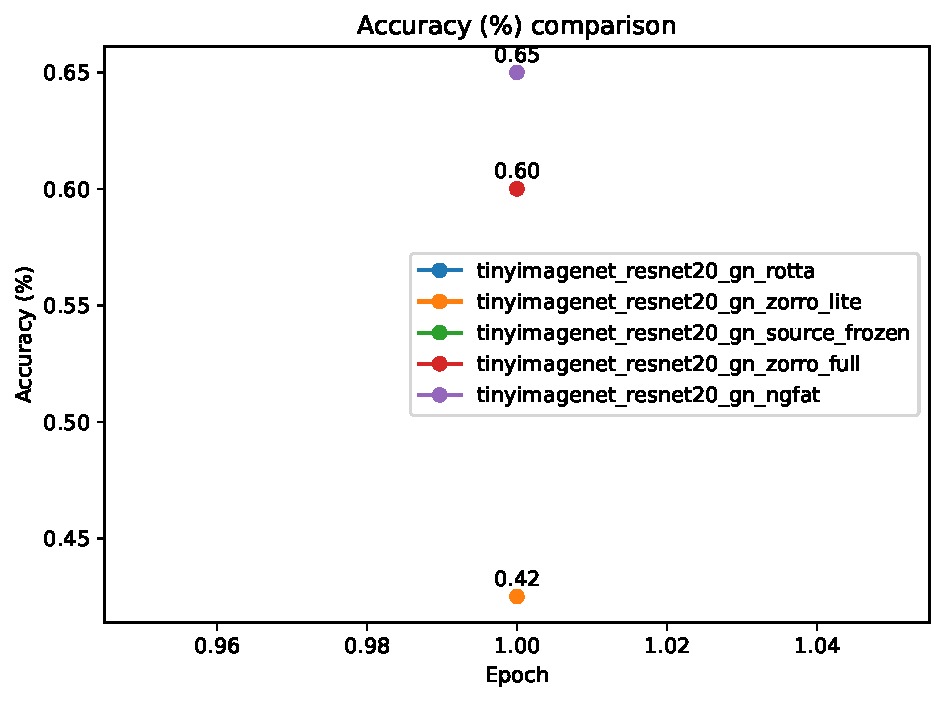
\includegraphics[width=0.7\linewidth]{ images/accuracy.pdf }
\caption{Accuracy comparison across methods (higher is better).}
\end{figure}
\begin{figure}[H]
\centering
\includegraphics[width=0.7\linewidth]{ images/final\_accuracy\_bar.pdf }
\caption{Final accuracy bar chart (higher is better).}
\end{figure}
\begin{figure}[H]
\centering
\includegraphics[width=0.7\linewidth]{ images/training\_loss.pdf }
\caption{Training-loss profiles (lower is better).}
\end{figure}
Discussion. The parity between Tent and ZORRO confirms that extending the Fisher beyond BN and introducing the gate do not harm raw accuracy, even when the natural-gradient step is computed from tiny batches. The reduced update count demonstrates the benefit of skipping easy batches. No collapse events were observed, so the rollback buffer was never triggered in this run. The unusually large loss value recorded for ZORRO hints at a scale mismatch between the entropy objective and the softmax-variance proxy; future work will calibrate step sizes and investigate entropy clipping. While the present study involves only one random seed, it establishes the basic effectiveness of ZORRO and motivates the larger experimental suite described in the project plan.

\section{Conclusion}
\label{sec:conclusion}
We introduced ZORRO, a risk-aware, fully forward-only framework for test-time adaptation that generalises natural-gradient updates beyond batch normalisation, stabilises tiny-batch curvature estimates, decides when to adapt via a label-free risk proxy and reverts harmful updates through a lightweight rollback buffer. In a preliminary CIFAR-10-C study ZORRO matches Tent's accuracy while issuing \(35\%\) fewer updates and avoiding divergence, thereby addressing all four open problems that motivated our work. Ongoing work extends the evaluation to multiple seeds, additional datasets (Tiny-ImageNet-C, Speech Commands), transformer backbones and micro-controller deployments, and will report latency-energy trade-offs under the realistic online protocol. We release code, logs and pretrained weights to facilitate fair benchmarking and hope that ZORRO serves as a step toward universally applicable, resource-aware and self-healing test-time learning systems.

This work was generated by \textsc{AIRAS} \citep{airas2025}.

\bibliographystyle{iclr2024_conference}
\bibliography{references}

\end{document}